\section{脚手架工程专项安全施工方案}
\subsection{编制依据}

脚手架的搭设规范主要参考自以下规范或文件:

(1) 《建筑施工脚手架使实用手册》

(2) 《建筑施工扣件式钢管脚手架安全技术规范》(JGJ130-2011)

(3) 《建筑施工高处作业安全规范》(JGJ80-2016)

(4) 《钢结构工程施工规范》(GB50755-2012)

(5) 《建筑结构荷载规范》(GB50009-2012)

(6) 《建筑施工手册》

(7) 《建设工程安全生产管理条例》(国务院令第 393 号)

\subsection{脚手架搭设要求}
\subsubsection{落地式脚手架搭设要求}

(1) 立杆基础设置应符合下列规定:\\

\quan{1} 基础应平整夯实,落地立杆应垂直稳放在金属底座或坚固底板上。

\quan{2} 立杆下部应设置纵横扫地杆。纵向扫地杆应采用直角扣件固定在距底座上面不大于 200mm 处的立杆上,

横向扫地杆应采用直角扣件固定在紧靠纵向扫地杆下方的立杆上。当立杆基础不在同一高度上时,必须将高处的纵向扫地杆向低处延长两跨与立杆固定,
高低差不应大于 1m。靠边坡上方的立杆轴线到边坡的距离不应小 于500mm.

\quan{3} 立杆基础外侧应设置截面不小于 200×200mm 的排水沟,保持立杆基础不积水,并在外侧 800mm 宽范围内采用混凝土硬化。

\quan{4} 外脚手架不宜支设在屋面、雨棚、阳台等处。确因需要,因分别对屋面、雨棚、阳台等部位的结构安全性进行验算,并在专项施工方案中明确。

\quan{5} 当脚手架基础下有设备基础、管沟时,在脚手架使用过程中不应开挖。当必须开挖时,应采取加固措施。

\quan{6} 钢管脚手架底步步距高度不大于 2m,其余不大于 1.8m,立杆纵距不大于 1.8m,横距不大于 1.5m.横距宜为 0.85m 或 1.05m.

\quan{7} 搭设高度超过 25m 须采用双立杆或缩小间距的方法搭设,双立杆中的副立杆的高度不应低于 3 步,且不少于6 m.

\quan{8} 底步立杆必须设置纵横向扫地杆,纵向扫地杆宜采用直角扣件固定在距底座上皮不大于 200mm 的立杆上,横向扫地杆也应用直角扣件固定在纵向扫地杆下方的立杆上。

\quan{9} 底排立杆、扫地杆、剪刀撑均漆黄黑或红白相间色。\\

\subsubsection{悬挑式脚手架搭设要求}

\quan{1} 挑架外挑梁或悬挑梁应积极采用型钢或定型桁架;

\quan{2} 悬挑型钢或悬挑架通过预埋与建筑结构固定,安装符合设计要求;

\quan{3} 挑架立杆与悬挑型钢连接必须固定,防止滑移;

\quan{4} 架体与建筑结构之间进行刚性拉结,按水平方向小于 7m、垂直方向等于层高设拉结点。

\quan{5} 挑架层层满铺脚手板,脚手板需要使用不小于 18\# 的铅丝双股并联绑扎不少于 4 点 ,要求交界处凭证,无探头板,不留空隙,
脚手片应保证完好无损,破损的及时更换;

\quan{6} 施工荷载应均匀堆放,并不能超过 $3.0kN/m^2$,建筑垃圾或不用的物料应及时清除;

\quan{7} 挑架外侧必须用经认证合格的密目式安全网封闭维护,安全网应用不小于 18\# 的铅丝张挂严密。且应将安全网挂在挑架立杆里侧,不得将网围在外侧;

\quan{8} 架体应该表面平整光滑,无锈蚀、裂纹、分层、压痕和硬弯,搭设架子前应该进行保养,除锈并统一上色,颜色应合理美观;

\quan{9} 脚手架搭设使用的扣件应该符合建设部《钢管脚手架扣减标准》,有合格证,扣件不得有裂纹、气孔、缩松、砂眼等锻造缺陷,贴合面应凭证,活动部位灵活,夹紧钢管时开口处最小距离不得小于 5mm;

\quan{10} 型钢宜采用 A3 号工字钢或槽钢。

\subsection{主要参数}

(1) 落地式、悬挑式脚手架搭设高度均为 18.00m。

(2) 脚手架采用外径 48.3mm,壁厚 3.6mm 的钢管。

(3) 架子立杆纵向间距 1.5m,内、外立杆横向距离 1.05m,内立杆距墙距离 150mm。

(4) 步高均按 1.5m 搭设。

(5) 小横杆间距 500mm,用扣件与立杆相连。

(6) 连墙杆水平方向每 4.5m 设一个,竖向每层应与建筑物相连。

(7) 扫地杆距垫块 200mm。

(8) 剪刀撑:应随外架的搭设而同时搭设,剪刀撑与地面的夹角一般为 45-60 度,
剪刀撑应连续设置不得中断。

(9) 脚手板:采用 50mm 厚木脚手板,且与小横杆固定。

(10) 安全网:架子外侧满挂密目尼龙安全网。

\subsection{脚手架计算书}
\subsubsection{双排脚手架安全性验算}

(1) 小横杆计算\\

按照 JGJ130-2011,小横杆按照简支梁进行强度和挠度计算,用大横杆支座的最大反力计算值作为小横杆集中荷载,在最不利荷
载布置下计算小横杆的最大弯矩和变形。\\

    \begin{figure}[thbp!]
        \centering
        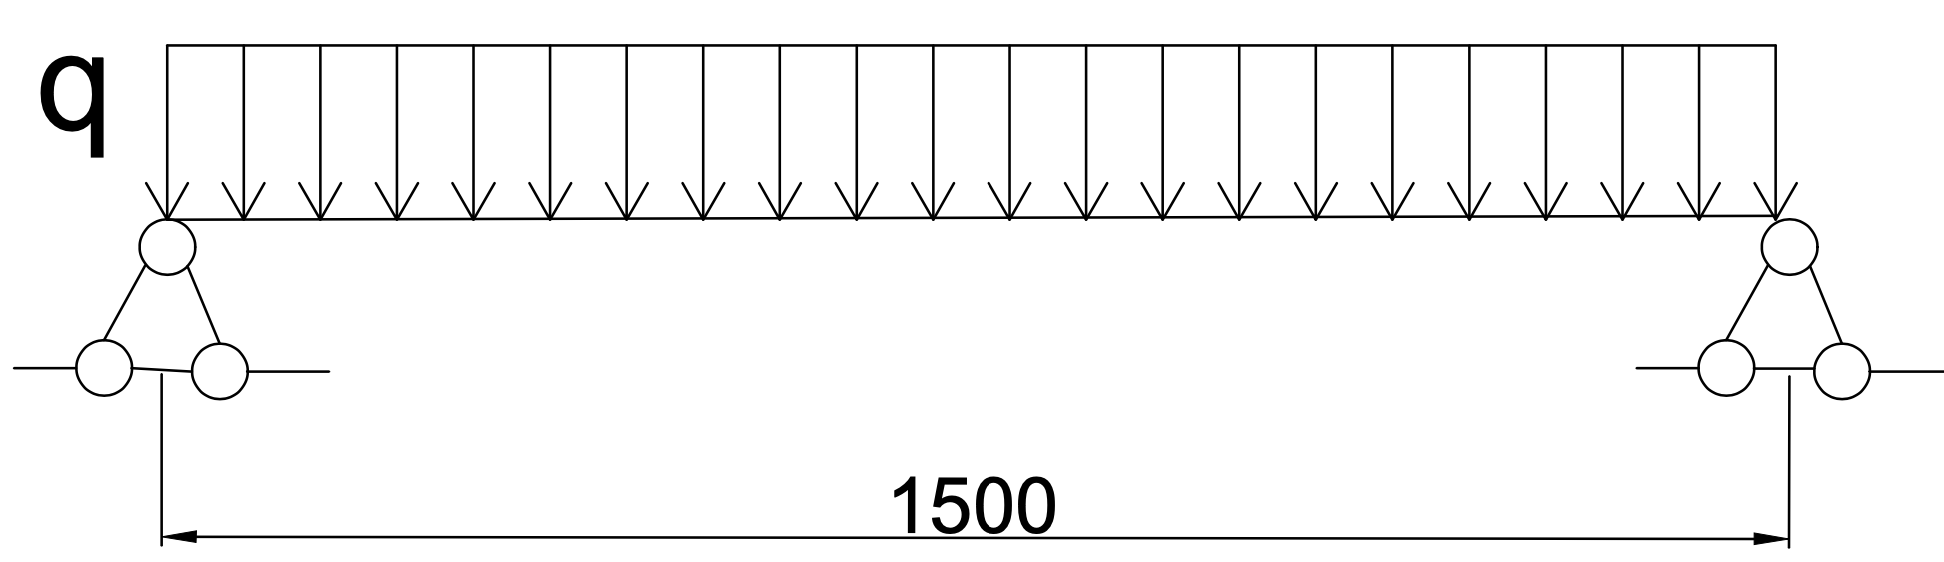
\includegraphics[width=0.8\linewidth]{figure/c4f1.png}
        \caption{小横杆受力简图}
        \label{fig:c4f1}
    \end{figure}

\quan{1} 均布荷载计算\\

小横杆的自重标准值:

$$p_1=0.0397 \times 1=0.0397 kN/m$$

脚手板的自重标准值:

$$p_2=\frac{0.35 \times 1.5}{2+1}=0.175 kN/m$$

施工荷载自重标准值:

$$Q=\frac{3 \times 1.5}{2+1}=1.5 kN/m$$

恒荷载做控制荷载设计值:

$$q_1=1.35\times(0.0397+0.175)+1.4\times 0.7\times 1.5=1.759 kN/m$$

活荷载做控制荷载设计值:

$$q_2=1.2\times(0.0397+0.175)+1.4\times 1.5=2.396 kN/m$$

\quan{2} 强度验算\\

恒荷载、活荷载二者取最大值,得出由活荷载做控制 $q=2.396 $kN/m。由于小横杆按照简支梁计算,故跨中弯矩值最大;

\begin{align}
    M_{max}=\frac{ql^2}{8}=\frac{2.396\times 1.05^2}{8}=0.33 kN\cdot m
\end{align}

式中:$q$ 为小横杆荷载设计值;$l$ 为小横杆计算跨度,即立杆横距。

计算最大应力,其中 $M_{max}$ 为最大弯矩, $W$ 为截面模量,取 $5.26 cm^3$,可得:

\begin{align}
    \label{fx:load}
    \sigma =\frac{M}{W}=\frac{0.33\times 10^6}{5.26\times10^3}=173.58N/mm^2
\end{align}

小横杆的计算强度 $173.58N/mm^2$ 小于小横杆的抗弯强度设计值 $205N/mm^2$,故强度满足要求!\\

\quan{3} 挠度验算\\

水平杆的挠度验算应满足 $v\leq [v] $,其中 $v$ 是挠度;小横杆的挠度计算式为:

\begin{align}
    V=\frac{5ql^4}{384EI}=\frac{5\times (0.397+0.175)\times 1050\times 10^4}{384\times 20.6\times 10^5\times 121870}=0.36 \text{mm}
\end{align}

式中 $E$ 为弹性模量,取$2.06\times 10^5$,$I$ 为惯性矩。

小横杆的最大挠度 0.36mm 小于 $1050.0/150=7.000$ 与 10mm,故挠度满足要求! \\

(2) 大横杆计算\\

按照《扣件式钢管脚手架安全技术规范》规定,大横杆按
照三跨连续梁进行强度和挠度计算,小横杆在大横杆的上面。
大横杆最大弯矩考虑均布荷载与集中荷载的最不利组合,且集中荷载、均布荷载最大弯矩值均出现在支座处,均上侧受拉。\\

\begin{figure}[thbp!]
    \centering
    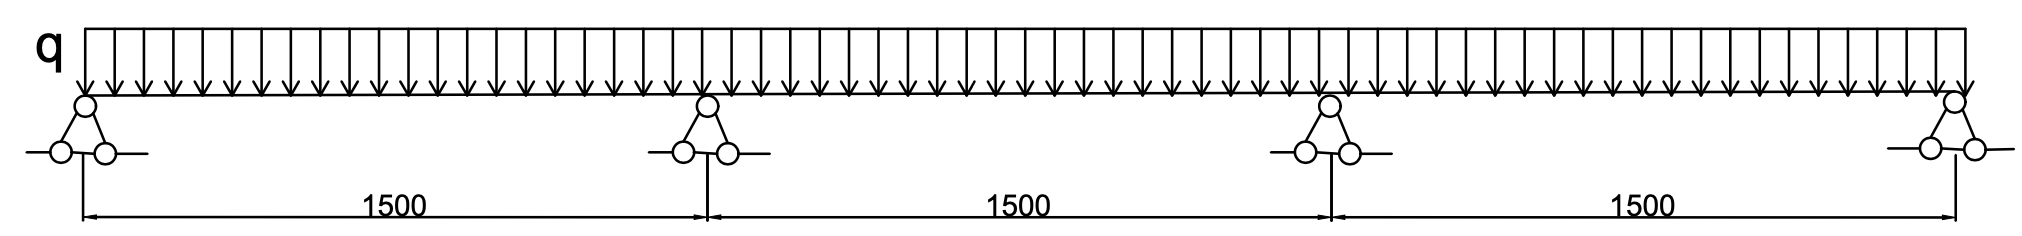
\includegraphics[width=1.0\linewidth]{figure/c4f2.png}
    \caption{大横杆受力简图}
    \label{fig:c4f2}
\end{figure}


\quan{1} 均布荷载值计算\\

小横杆的自重标准值:

$$p_1=0.0397 \times 1.05=0.042 kN/m$$

脚手板的自重标准值:

$$p_2=\frac{0.35 \times 1.5\times 1.05}{2+1}=0.184 kN/m$$

施工荷载自重标准值:

$$Q=\frac{3 \times 1.5\times 1.05}{2+1}=1.575 kN/m$$

恒荷载做控制荷载设计值:

$$q_1=\frac{[1.35\times(0.042+0.184)+1.4\times 0.7\times 1.575]}{2}=0.96 kN/M$$

活荷载做控制荷载设计值:

$$q_2=\frac{[1.2\times(0.042+0.184)+1.4\times 1.575]}{2}=1.27 kN/M$$

\quan{2} 强度验算\\

恒荷载、活荷载二者取最大值,得出由活荷载做控制 $q=1.27 kN/M$ 。由于大横杆最大弯矩考虑均布荷载与集中荷载的最不利组合,
且集中荷载、均布荷载最大弯矩值均出现在支座处,则

\begin{align}
    M_{max}=0.1pl^2+0.289ql
\end{align}

根据公式 \ref{fx:load} 可得 $\sigma =(0.503\times 10^6)/(5.26\times 10^3)=95.63 N/mm^2 \leq f=205 N/mm^2$\\
故强度满足要求!\\

\quan{3} 挠度验算\\

大横杆最大挠度考虑均布荷载与集中荷载的最不利组合;故荷载的最大挠度为:

\begin{align}
    V_{max}=\frac{0.99pl^4+2.76ql^3}{100EI}
\end{align}

带入数值得

$$V_{max}=\frac{0.99\times 0.397\times 1500^4+2.76\times (0.042+0.184)\times 1500^3/2}{100\times 2.06\times 10^5\times 121870}=0.792$$

大横杆的最大挠度 $0.792mm$ 小于 $1050.0/150=7.000$ 与 $10mm$,故挠度满足要求! \\

(3) 扣件抗滑计算\\

按照规范,直角,旋转单扣件承载力设计值取 $8.00kN$,纵向或横向水平杆与立杆连接时,扣件的抗滑承载力按照 《建筑施工扣件式钢管脚手架安全技术规范》 计算:

\begin{align}
    \label{fx:rc}
    R \leq R_c
\end{align}

竖向作用力设计值 $R$ 计算:

\quan{1} 大横杆自重标准值:$P_1=0.0397×1.5=0.059kN$

\quan{2} 小横杆自重标准值平均分配到两侧立杆:$P_2=0.0397×1.05/2=0.02kN$ 

\quan{3} 脚手板自重标准值平均分配到两侧立杆:$P_3=0.35×1.05×1.5/2=0.27kN$ 

\quan{4} 活荷载自重标准值平均分配到两侧立杆:$Q=3×1.05×1.5/2=2.36kN$

根据公式 \ref{fx:rc} ,荷载设计值:

$$R=1.2×(0.059+0.02+0.27)+1.4×2.36=3.72kN<R_c=8.0kN$$

故单扣件抗滑移能力可以满足要求。\\

(4 )立杆稳定性验算\\

根据 《建筑施工扣件式钢管脚手架安全技术规范》 ,立杆的稳定性应按照下列公式计算:

不组合风荷载时:

\begin{align}
    \label{fx:nw}
    \frac{N}{\varphi A}\leq f
\end{align}

组合风荷载时:

\begin{align}
    \label{fx:w}
    \frac{N}{\varphi A}+ \frac{M_W}{W}\leq f
\end{align}

式中:

$N$ 为计算立杆的轴向设计值;

$\phi$ 为轴心受压构件的稳定系数,根据规范取值;

$\lambda$ 为长细比,$\lambda =l_0/I$;

$l_0$ 为计算长度,根据规范计算;

$i$ 为截面回转半径,根据规范取值;

$A$ 为立竿截面面积,根据规范取值;

$M_W$ 为计算立杆段由风荷载设计值产生的弯矩,根据规范计算;

$f$ 为钢材的抗压强度设计值,根据规范取值;

按照组合风荷载计算,立杆的轴向设计值应该为:

\begin{align}
    \label{fx:Nzhou}
    N=1.2(N_{G1k+G2k})+0.9\times 1.4\sum N_{Qk}
\end{align}

式中:

$N_{G1k}$ 为脚手架结构自重产生的轴向力标准值; 

$N_{G2k}$ 为构配件自重产生的轴向力标准值;

$\sum N_{Qk}$ 为施工荷载产生的轴向力标准值总和,内、外立杆割按一纵距内施工荷载
总和的 $1/2$ 取值。

可得:

$N_{G1k}=18.0\times 0.144=2.59 kN$

$N_{G2k}=0.5\times (1.05+0.15)\times 1.5\times 2\times 0.35+1.5\times 2\times 0.16+1.5\times 18\times 0.01=1.41 kN$

$N=1.2\times (2.59+1.41)+0.85\times 1.4\times 4.5=10.15 kN$

立杆段由风荷载设计值产生的弯矩为:

\begin{align}
    M_W=0.9\times 1.4M_{Wk}=0.9\times 1.4\omega _kl_ah^2/10=0.21kN\cdot m
\end{align}

可得立杆稳定性的设计值为

$$\frac{10150}{0.265×5.06×10^2}+\frac{210000}{5.26×10^3}=115.6 N\cdot mm \leq f=205 N\cdot mm$$

故立杆的稳定性满足要求。\\

(5) 连墙件计算\\

连墙件杆件的强度应满足:

\begin{align}
    \sigma =\frac{N_l}{A_c}\leq 0.85f
\end{align}

稳定性应满足:

\begin{align}
    \label{fx:stb}    
    \frac{N_l}{\phi A}\leq 0.85f
\end{align}

\begin{align}
    N_l=N_{lw}+N_0
\end{align}

式中:

$A_c$ 为连墙件的净截面面积;  

$N_l$ 为连墙件轴向力设计值;   

$N_{lw}$ 为风荷载产生的连墙件轴向力设计值,按照公式 $N_{lw}=1.4\cdot w_k\cdot A_w$ 计算;

$N_0$ 为连墙件约束脚手架平面外变形所产生的轴向力,双排架取 $3.0kN$。

计算连墙件强度: 

$$\sigma=\frac{1.4×0.5×6×1.5×1.5+3}{506}=24.6 N/mm^2<0.85f=174 N/mm^2$$

故强度满足设计要求。

计算连墙件稳定性:

构件长细比为 $\lambda =l_0/I=150/1.59=9.43$,查表可得 $\phi=0.976$

根据公式 \ref{fx:stb} ,代入数据:

$$\sigma =\frac{12450}{0.976\times 1912}=6.67 N/mm^2<0.85f=174 N/mm^2$$

故稳定性满足设计要求。\\

(6) 地基承载力计算\\

立杆基础底面平均压力应满足下式:

\begin{align}
    p_k=\frac{N_k}{A} \leq f_g
\end{align}

\begin{align}
    f_c=k_c\times f_{g}
\end{align}

式中:

$p_k$ 为立杆基础底面处的平均压力标准值;   

$N_k$ 为上部结构传至立杆基础顶面的轴向力标准值; 

$A$ 为基础地面面积;                       

$f_g$ 为地基承载力特征值(kPa);$k_c$ 取 0.4。

可得 $N_{G1k}=H\times G_k=18.0\times 0.1444=2.59kN$、$N_{G2k}=1.41kN$、$N_{Qk}=4.54kN$;
按照公式 \ref{fx:Nzhou} 可得

$N=1.2\times (2.59+1.41)+1.4\times 4.54=9.9kN $

$Pk=9.9/(0.5×0.5)=39.6kN/m^2\leq f_g/0.4=99.4kN/m^2$

故地基承载力满足设计要求。\\

(7)最大允许搭设高度计算\\

双排脚手架的可搭设高度 $[H]$ 应按照下列公式计算,并取最小值:

不组合风荷载时:

\begin{align}
    \label{fx:bzh} 
    [H]=\frac{\phi Af-(1.2N_{G2k}+1.4\sum N_{Qk})}{1.2g_k}
\end{align}

组合风荷载时:

\begin{align}
    \label{fx:zh} 
    [H]=\frac{\phi Af-[1.2N_{G2k}+0.9\times 1.4(\sum N_{Qk}+\frac{M_{wk}}{W}\phi A)]}{1.2g_k}
\end{align}

式中:

$[H]$ 为脚手架最大允许搭设高度;

$g_k$ 为立杆承受的每米结构自重标准值,查规范可得 $g_k=0.1444kN/m$;

$A$ 为脚手架钢管截面面积; 

$f$ 为钢材强度设计值; 

$W$ 为截面模量。\\

当不组合风荷载时,将数据带入公式 \ref{fx:bzh} 得:

\begin{align*}
    [H] &=\frac{0.265\times 5.06\times10^{-4}\times 2.05\times 10^5-(1.2\times 1.41+1.4\times 4.5)}{1.2\times 0.1444}\\
    &=109.1m
\end{align*}

当组合风荷载时,将数据带入公式 \ref{fx:zh} 得:

\begin{align*}
[H] &=\frac{0.265\times 5.06\times10^{-4}\times 2.05\times10^5-[1.2\times 1.41+0.9\times 1.4\times(6.18+\frac{0.22\times 0.265\times 5.06\times 10^{-4}}{5.26\times 10^{-6}})]}{1.2\times 0.1444}\\
&=85m
\end{align*}

取最大允许搭设高度 50m,18.0m 符合要求。

\subsection{脚手架质量验收}

(1) 脚手架搭设前,对进入现场的各种构配件应按下列规定进行检查验收,不合格的应及时清除出场;
构配件应有相应的产品标识及产品质量合格证;构配件应有相应的技术参数及产品使用说明书;当对构配件质量有疑问时,应进行质量抽检和实
验。

(2) 脚手架在悬挑层顶梁板浇筑后及脚手架搭设前;作业层上施加荷载前;每搭设完两层后;达到设计高度后;遇有六级强风及以上风或大雨后;停
用超过一个月时应该进行检查与验收,按规定对脚手架工程的质量进行检查,合格后方可交付使用;

(3) 架子搭设和组装完毕,使用前必须由项目经理、技术负责人、项目安全负责人、架子班长等人员组成验收小组,
进行验收,并填写验收单。

(4) 脚手架使用期间必须设专人经常检查,符合要求后,必须经过项目经理签字批准,才能使用;
不合格部位必须及时修复或更换,符合规定后,方准许继续使用。 

\subsection{安全技术措施}
\subsubsection{脚手架搭设安全技术措施}

(1) 钢管架应设置避雷针,分置于主楼外架转角立杆之上,并联通大横杆,形成避雷网络。

(2) 脚手架不得搭设在距离外电架空线路的安全距离内,并做好可靠的安全接地处理。

(3) 定期检查脚手架,发现问题和隐患,在施工作业前应及时维修加固。

(4) 脚手架严禁钢木混用。

(5) 严禁脚手板存在探头板,铺设脚手板以及多层作业时,应尽量使施工荷载内、外传递平衡。

(6) 结构外脚手架每支搭一层,支搭完毕后,经项目部安全员验收合格后方可使用。任何班组长和个人,未经同意不得任意拆除脚手架部件。

(7) 脚手板不得集中堆料施荷,施工荷载不得大于 $4kN/m^2$。

\subsubsection{脚手架拆除安全技术措施}

(1) 拆除前应全面检查脚手架,根据检查结果指定施工计划,并报请批准;

(2) 拆架时应划分作业区,周围设置围栏竖立警示标志,地面应有专人指挥并禁止非作业人员进入;

(3) 拆架程序应先上后下,先搭后拆。即先插拉杆、脚手板、剪刀撑、斜撑;后拆小横杆、大横杆、立杆等,并按照一步一清的原则严格执行,禁止上下同时拆架;

(4) 连墙件应随拆除进度逐层拆除,拆除时应用临时支撑固定,然后才能拆除;

(5) 作业时应统一指挥,上下呼应,动作协调。当解开与人有关的结扣时,应先通知对方,以防坠落;

(6) 拆架时严禁触碰脚手架附近的电源线,以防触电;

(7) 拆架过程中不得中途换人,如必须换人必须将拆除情况交代清楚;

(8) 拆下的材料严禁抛掷,运至地面后应分类堆放,当天拆下的材料应及时运走;

(9) 高层建筑脚手架拆除时应配备良好的通讯设备;

(10) 强风、暴雨、暴雪等恶劣条件下禁止拆架,夜间不得进行拆架作业。